\chapter{Scalability Approaches}
\label{ch:Scalability Approaches}

Some of the scaling approaches from differents papers are discussed in the below section

\section{Service replication}
Service replication: Service replication is a technique for cloning services that are already running on the other nodes to optimize the service load over the nodes without affecting operations in progress. Replicated services secure additional resources provided by the new nodes for handling larger service load. In other words, service replication enhances service scalability and reduces the risk of QoS degradation by handling larger service loads.To perform a case study, they firstly set a service load as variable. The service load is a number of service invocations within a unit time. For the case study, we set 500ms as the unit time. That is, if ten invocations occur within 500ms, then the service load is 10. To show an effectiveness of service replication, they simulate the service replication scheme for the seventeen different volumes of service load. On each service load, they compare (1) conventional service system with (2) service replication scheme in terms of average response time
\cite{falatah_cloud_2014}.

\section{Service Migration}

Service migration is a scheme for placing a service to other node when a particular node cannot provide high QoS cause by a physical problem, software problem, or a physical distance between consumers and providers. After service migration, the migrated service performs the same role of the unstable service, and the unstable node is removed from the list of service nodes. This is a way to reduce overall QoS degradation by firstly excluding the unstable node\cite{lee_software_2010}.


\section{Proactive scaling}

Proactive scaling is usually done in a cloud by scaling at predictable, fixed intervals or when big surges of traffic requests are expected. A well-designed proactive scaling system enables providers to schedule capacity changes that match the expected changes in application demand. To perform proactive scaling, they should first understand expected traffic flow. This simply means that they should understand (roughly) how much normal traffic deviates from agency expectations. The most efficient use of resources is just below maximum agency capacity, but scheduling things that way can create problems when expectations are wrong \cite{falatah_cloud_2014}\cite{reese_cloud_nodate}



\section{Reactive scaling}

A reactive scaling strategy can meet this demand by adding or removing, scaling up or down resources. Periodic acquisition of performance data is important both to the cloud provider and to the cloud agencies for maintaining QoS. In addition, reactive scaling enables a provider to react quickly to unexpected demand. The crudest form of reactive scaling is utilization-based.\cite{falatah_cloud_2014}\cite{reese_cloud_nodate}

\section{Service System Scaling - Dynamic node scaling}
According to \cite{lee_software_2010} service system consists of multiple nodes which are distributed over the Internet. Therefore, service consumers do not know physical location of service node which they use. To construct scalable service system, management components which are able to monitor current status of nodes and manage them are needed. Therefore, we propose two key components to manage service scalability such as Global Scalability Manager (GSM) and Regional Scalability Manager (RSM). 
GSM is a central component of a service system to manage service scalability. GSM takes a role to balancing service load over the service system. To enable this, GSM acquires current status of nodes which are registered into the service system, and plans a scalability assuring method. Based on the method, GSM instructs relevant functionality. RSM is a management component installed on a node. A RSM observes its node status and delivers it to GSM, and also performs scalability assuring scheme based on the instructions from GSM. Using these two components, our service system provides a function to add or remove new nodes at run-time called as dynamic node management.

\subsection{Service Scalability Assuring Process}


\begin{itemize}
	

\item Step 1 is to define quality metrics for measuring service scalability. For example, throughput is a metric which measures the efficiency of handling service invocations within a given time. Metrics defined in this step are used in two ways; (1) as the basis for deciding raw data items to collect from services, and (2) for computing scalability in step 3. Representative metrics for scalability are given in section 3. 

\item Step 2 is to acquire the set of raw data items from monitored services. Various techniques such as \cite{Artaiam2008EnhancingSQ} and \cite{hutchison_monitoring_2007} can be used to acquire such data elements. 



\item Step 3 is to compute scalability metrics. If the computed metrics reveal an acceptable scalability level, the control goes back to step 2 and repeat applying steps 2 and 3. If the resulting metrics shows a need to take actions to remedy the low scalability, steps 4, 5, and 6 are performed. 


\item Step 4 is to devise a remedy plan for enhancing suffered scalability based on the current states of monitored service. In section 6, we propose scalability assuring schemes which can be included in the plan. Depending on the complexity and nature of the suffered service, one or more schemes can be applicable. 


\item Step 5 is to run the selected scalability assuring schemes according to the plan. Many, if not all, of the schemes should be able to run without human administrators’ intervention to be autonomous, as proposed in section 6. 

\item Step 6 is to analyze the result of applying the remedy plan and to learn from the whole process of enhancing scalability. If the result is shown to be effective, the remedy plan and the suffered situation are recorded for further applications; making the whole scalability framework more intelligent
\begin{figure}[h]
	\centering
	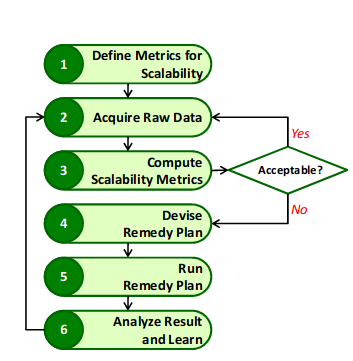
\includegraphics[width=0.7\linewidth]{figures/ServiceScalability}
	\caption{Service scalability Assuring Process from \cite{lee_software_2010}}
	\label{fig:servicescalability}
\end{figure}

\end{itemize}


\section{Scalability of Distributed Systems}

Another approach in \cite{jogalekar_evaluating_2000} is a very general family of metrics can be based on the following definition:

\begin{figure}[h]
	\centering
	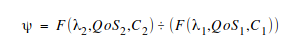
\includegraphics[width=0.5\linewidth]{figures/scalingformula}
	{\caption*{}}
	\label{}
\end{figure}
where F evaluates the performance and the economy of operation of the system at two different scales of deployment. The reasoning behind the selection of variables in F is, that: lambda evaluates the rate of providing valuable services to users, which is related to revenue capability, QoS is a set of parameters which evaluate the quality of the service seen by users. C reflects the cost of providing service.

Scaling Strategy : A strategy for scaling up a system will be defined by a scaling factor k and a set of scaling variables which are functions of k. They express the strategy as a scaling path in a space in which they are the coordinates.

\begin{figure}[h]
	\centering
	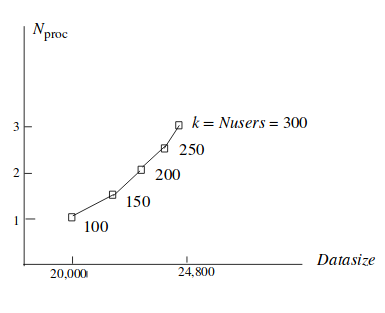
\includegraphics[width=0.7\linewidth]{figures/scalegraph}
	\caption{Scaling variables and the scaling path from \cite{jogalekar_evaluating_2000}}
	\label{fig:scalegraph}
\end{figure}

\newpage

\section{Hierarchical Service Placement}
In the centralized model, the service orchestrator has a detailed view of all Execution Zones(EZs).It may be impractical, for scalability reasons, for a globally centralised placement algorithm to maintain detailed knowledge of all users and all EZs and so here the author investigates a hierarchical solution where the overall orchestration domain is split into geographical sub-domains. The details are provided in .

In this model the high-level orchestrator has limited visibility of Execution Zone(EZ - Services will be deployed in datacenters/clouds called EZ) and user demands within a sub-domain - it sees only the aggregate of user demands and the aggregate of EZ capacities within a particular sub-domain. The high-level orchestrator places service instances at the coarse granularity of sub-domain only and subsequently each sub-domain orchestrator undertakes a further placement algorithm with the scope of that sub-domain only to determine in which specific EZs what quantity of service instances should be placed to supply the required number of session slots to meet the specific detailed demand pattern of user requests within that sub-domain.
\paragraph{}There are many ways of sub-dividing an overall orchestration domain into sub-domains. One option is to map sub-domains onto the same geographical area covered by resolution domains: the entity responsible for resolving user requests to EZs with available session slots. Equating sub-domains for orchestration and service placement purposes with resolution domains is not essential as other coarser or finer grained sub-domains could be considered
 \cite{maini_hierarchical_2016}.
